% =====================================================================
% STALE AS OF 2026-10-06. DO NOT \input THIS WITHOUT REWRITING THE NUMBERS.
% =====================================================================
%
% This section was written mid-campaign and its coefficients were fitted ACROSS
% the knee, which overstates c and understates F from one cause. The campaign
% then re-measured both BELOW the knee on the shipped code and ran four
% optimisations (T7a, T8 landed; T5, T6, T7b did not). Superseded numbers:
%
%     quantity              this section     measured, final
%     c at the target       1.736 ms/rider   0.61     (below the knee, L=80)
%     F at the target       5.90 ms          4.24     (after T8, +-0.5)
%     gain at C2C           1.22x            1.20x    (anchor L70/8192)
%
% Two CLAIMS in the prose change sign or strength, not just magnitude:
%
%   1. "the interconnect divides exactly one [cost], and at the operating point
%      that one is under a tenth of the total" -- this SURVIVES and in fact
%      strengthens: below the knee the transfer hides COMPLETELY. The minbytes
%      arm (bytes removed, launches kept) moves c by -0.010 ms. c is exposed
%      work only: launches plus host bookkeeping.
%   2. Any statement that c is the binding constraint is WRONG. c clears the
%      T0/B budget by 5.5x. F is what binds, and F is now 56% a single
%      identified item: the per-layer second attention call.
%
% AUTHORITATIVE SOURCE for every number above:
%     paper/OVERHEAD_CHARACTERISATION.md   (the report, with provenance)
%     paper/model/overhead_model.py        (dict FINAL, func closing_state)
% Do NOT re-derive from COEFF in that module -- COEFF is the across-the-knee fit
% and is kept only so the superseded reasoning stays auditable.
%
% Overhead characterisation. NOT yet \input into main.tex: the body already
% runs long against the MLSys limit, so wiring this in is a page-budget
% decision rather than a build one. One \input line in main.tex adds it.
%
% CONVENTION: every numeric claim carries a "% src:" pointer, ASCII only.
\section{Where the overhead comes from, and what a faster interconnect can do}
\label{sec:overhead}

A host-tier request --- a \emph{rider} --- buys capacity by keeping its KV in
host memory and re-streaming it across the CPU--GPU link once per decode step.
Whether this is profitable turns on a single quantity: the step time a rider
adds. The design's premise is that a faster interconnect shrinks that quantity,
admits more riders, and so raises throughput. This section tests that premise by
decomposing the added step time into terms that scale with different variables,
and asking of each term whether a faster link touches it at all.

The result is that the premise holds, but not for the reason the design assumed.
Of the four costs a rider imposes, the interconnect divides exactly one, and at
the operating point the paper targets that one is under a tenth of the total.
What the interconnect actually buys is not a cheaper rider but a larger number
of \emph{admissible} riders, and the two are not interchangeable.

\subsection{What a rider costs, structurally}
\label{sec:overhead:anatomy}

\emph{Question: what work does a rider create, and what does each piece of that
work scale with?} The decomposition below is not a fitting convenience; it falls
out of the mechanism, and it is what makes the measurements in
\S\ref{sec:overhead:c} identifiable.

A rider's KV lives in pinned host memory as a per-layer mirror, laid out
block-major, with each request allocated one \emph{contiguous extent} of blocks.
On the device the design keeps a small rolling window of $k$ slots rather than a
full copy. A decode step then walks the $L$ layers, and at layer $\ell$:

\begin{enumerate}
\itemsep2pt
\item the cohort's layer-$\ell$ KV is copied host-to-device into a rolling slot,
      one \texttt{cudaMemcpyAsync} per contiguous run per tensor;
\item attention runs against that slot together with the resident requests' KV;
\item the new token's layer-$\ell$ KV is folded back into both the rolling slot
      and the host mirror, so the next step re-streams a current history.
\end{enumerate}

Figure~\ref{fig:overhead:anatomy} shows one layer of this walk and where each
cost class arises. Because the mirror is block-major and each request owns a
contiguous extent, a request's active blocks form one ascending run, so step~1
is a handful of large contiguous copies rather than a gather. This matters: an
earlier layout forced a CPU staging copy per layer and ran at 6.4\,GB/s, which
was the binding constraint on the whole path.

\begin{figure}[t]
\centering
\small
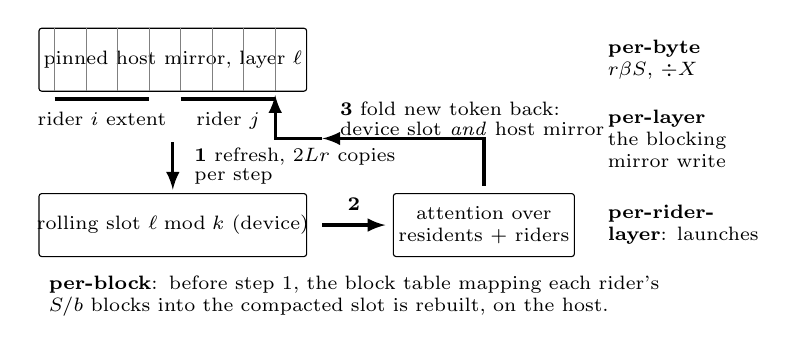
\begin{tikzpicture}[x=1mm,y=1mm,font=\scriptsize]
  % host mirror, block-major, one contiguous extent per request
  \draw[rounded corners=1pt] (0,26) rectangle (34,34);
  \node at (17,30) {pinned host mirror, layer $\ell$};
  \foreach \x in {0,4,8,12,16,20,24,28}
    \draw[gray] (\x+2,26) -- (\x+2,34);
  \draw[very thick] (2,25) -- (14,25);
  \node[anchor=north] at (8,24.6) {rider $i$ extent};
  \draw[very thick] (18,25) -- (30,25);
  \node[anchor=north] at (24,24.6) {rider $j$};

  \draw[-latex,very thick] (17,19.5) -- (17,13.5);
  \node[anchor=west,align=left] at (18.5,16.5)
    {\textbf{1} refresh, $2Lr$ copies\\[-1pt] per step};

  \draw[rounded corners=1pt] (0,5) rectangle (34,13);
  \node at (17,9) {rolling slot $\ell \bmod k$ (device)};

  \draw[-latex,very thick] (36,9) -- (44,9);
  \node[anchor=south] at (40,9.6) {\textbf{2}};
  \draw[rounded corners=1pt] (45,5) rectangle (68,13);
  \node[align=center] at (56.5,9) {attention over\\ residents $+$ riders};

  \draw[-latex,very thick] (56.5,14) -- (56.5,20) -- (36,20);
  \node[anchor=west,align=left] at (37,22.5)
    {\textbf{3} fold new token back:\\[-1pt] device slot \emph{and} host mirror};
  \draw[-latex,very thick] (36,20) -- (30,20) -- (30,25.5);

  \node[anchor=west,align=left] at (71,30)
    {\textbf{per-byte}\\ $r\beta S$, $\div X$};
  \node[anchor=west,align=left] at (71,20)
    {\textbf{per-layer}\\ the blocking\\ mirror write};
  \node[anchor=west,align=left] at (71,9)
    {\textbf{per-rider-}\\\textbf{layer}: launches};
  \node[anchor=west,align=left,text width=82mm] at (0,0)
    {\textbf{per-block}: before step 1, the block table mapping each rider's
     $S/b$ blocks into the compacted slot is rebuilt, on the host.};
\end{tikzpicture}
\caption{One layer of a decode step with $r$ riders, and where each cost class
of Table~\ref{tab:overhead:classes} arises. Steps 1--3 repeat for all $L$
layers; the per-block rebuild happens once per step, before the layer walk. Only
the per-byte class is divided by link bandwidth $X$.}
\label{fig:overhead:anatomy}
\end{figure}

\begin{table}[t]
\centering
\small
\begin{tabular}{@{}llll@{}}
\toprule
cost class & count per step & scales with & link? \\
\midrule
per-layer        & $L$             & depth           & no \\
per-rider-layer  & $2 L r$         & depth, riders   & no \\
per-block        & $r \cdot S / b$ & riders, context & no \\
per-byte         & $r \cdot \beta S$ & riders, context & \textbf{yes} \\
\bottomrule
\end{tabular}
\caption{The four classes of work a cohort of $r$ riders at context $S$ creates
in a step, for a model of $L$ layers with KV block size $b$ and $\beta$ bytes of
KV per token. Only the last is divided by link bandwidth. The first lands in the
fixed cost $F$; the other three land in the per-rider cost $c$.}
\label{tab:overhead:classes}
\end{table}

Table~\ref{tab:overhead:classes} names the four classes and their scaling.
Concretely:

\paragraph{Per-layer work} is anything done once per layer however many riders
are present: the rolling-slot bookkeeping, the event chain that overlaps the
next layer's copies, and --- as \S\ref{sec:overhead:F} shows --- a
host/device synchronisation that turns out to dominate it. Being independent of
$r$, it appears as a \emph{fixed} charge paid as soon as any rider exists.

\paragraph{Per-rider-per-layer work} is the copy \emph{launches}: two
\texttt{cudaMemcpyAsync} per rider per layer, so $2 L r$ per step, which is
$1024$ at $L{=}64$ and $r{=}8$. This is launch overhead, not transfer time, and
it is proportional to depth but independent of context.

\paragraph{Per-block work} is host bookkeeping proportional to the number of KV
\emph{blocks} a rider owns, $S/b$: principally rebuilding the block table that
maps each rider's blocks into the compacted rolling region. It is pure CPU work
that no interconnect touches.

\paragraph{Per-byte work} is the transfer itself, $r \beta S$ bytes per step,
and the only class a faster link divides.

Per-block and per-byte both scale with $S$, which is precisely why they cannot
be separated by varying context: at a fixed block size, doubling $S$ doubles
blocks \emph{and} bytes. Distinguishing them requires varying $b$ at fixed $S$,
which changes the block count while leaving the byte volume untouched, and this
experiment is the reason the decomposition is identifiable at all.

\subsection{Method}
\label{sec:overhead:method}

\emph{Two methodological problems had to be solved before any of this is
measurable, and they shaped every number that follows.}

\paragraph{Isolating the decode node.} Overhead attributable to riders is easily
confused with queueing on the prefill side. Every measurement here runs a
prefill/decode-emulated configuration with the host tier on the decode node, and
every measured step is checked against four conditions: zero prefill tokens,
nothing waiting in the queue, the admitted tier counts matching the request
exactly, and the running cohort equal to residents plus riders. Points failing
the gate are discarded rather than adjusted. The gate is not ceremony: one
archived curve in our own earlier data charges a growing resident batch to
riders, because a request the controller refuses as a rider is still served as a
resident, and the gate's tier-count assertion is what catches it.
% src: paper/data/overhead/MANIFEST.json @ 908d2a773

\paragraph{The knee, and why short contexts are the enabling trick.} A rider's
transfer hides inside compute until the cohort's aggregate transfer exceeds the
step, at which point the step \emph{is} the transfer. The crossover sits at
\begin{equation}
r^{*} = \frac{T_0 X}{\beta S},
\label{eq:overhead:knee}
\end{equation}
for a rider-free step time $T_0$ and link bandwidth $X$. Below $r^{*}$ the added
time is the \emph{exposed} critical-path cost, which is exactly the quantity a
faster link leaves behind; above it, the measurement reads bandwidth and nothing
else. On A100/PCIe at the paper's context this knee sits near two riders, which
is why a rider axis has previously been impossible to fit.

Equation~\ref{eq:overhead:knee} also shows the way out: $r^{*}$ varies as $1/S$,
so \emph{shortening} the context widens the rider axis on fixed hardware. At
$S{=}512$ the knee is 8 riders and at $S{=}256$ it is 14, which turns a
two-point axis into an eight-point one.
% src: paper/data/overhead/02_law/A_c512.json @ 908d2a773
Short contexts are a measurement instrument here, not an operating point, and
every fit below is confined to points beneath the knee. Pooling the two regimes
is how an automated model search in an early round of this work selected a
spurious superlinear term over the affine law while passing its held-out check.

\paragraph{Estimator and instrumentation.} Step time is taken directly, as the
median interval over a steady window, rather than by differencing a long run
against a short one. The two agree to 0.2\% below the knee but diverge by
$-2.7$\% at the largest cohort, where the admission ramp outlasts the short run
and contaminates the difference. Instrumentation is split in two: counters and
host-side timers that cost 0.053\% of a step and are always on, and anything
requiring a device-side wait, which is excluded from every absolute coefficient
reported here. The exclusion is not precautionary. Phase timers bracketing a
\emph{blocking} copy accounted for 214--304\% of the quantity they were meant to
partition, so the costs in \S\ref{sec:overhead:F} are obtained by differencing
configurations instead.
% src: paper/data/overhead/01_perturbation/t0_c512.json @ 908d2a773

\subsection{The overhead law}
\label{sec:overhead:law}

\emph{Claim under test: the added step time is affine in the rider count, with a
fixed part and a per-rider part.}

Writing $\Delta T(r)$ for the step time at $r$ riders minus the step time at
none, the data below the knee are described by
\begin{equation}
\Delta T(r) = F + c\,r ,
\label{eq:overhead:law}
\end{equation}
with a maximum residual of 0.42\,ms on a $\Delta T$ of 17.6\,ms at $S{=}512$
over eight rider counts.
% src: paper/data/overhead/02_law/A_c512.json @ 908d2a773
Model selection over all subsets of the candidate terms, with bootstrap
intervals and a fifth of the points held out, retains no superlinear term, and
the law predicts the step to the millisecond at a cohort and byte volume where
earlier code did not complete at all.
% src: paper/data/overhead/04_stall/s512_xhi.json @ 908d2a773

Two qualifications matter.

First, the affine form is not assumed; it is what survives an attempt to
refute it. Riders might be expected to \emph{share} part of their cost, since
$2 L r$ back-to-back copies could queue more efficiently than one does alone,
which would make $\Delta T$ concave. Fitting $\Delta T = F + c\,r^{\alpha}$ does
return $\alpha = 0.69$ at $S{=}512$, with an $F$-test rejecting $\alpha{=}1$
($F(1,5) = 10.28$), a bootstrap putting $P(\alpha<1)$ at 98\%, affine residuals
negative at both ends of the rider range and positive in the middle, and the
estimate surviving leave-one-out within $0.52$--$0.74$.

\emph{All five of those checks are nonetheless uninformative here}, and the
reason is worth stating because it generalises. The three-parameter fit is
nearly unidentified: at the first rider point $F$ is roughly 95\% of
$\Delta T$, so $F$ and $c\,r^{\alpha}$ trade off against one another with
almost no leverage on the exponent. Every check above conditions on the fit
window and the points inside it, so none of them can detect that the estimate
moves wholesale when the window changes --- which it does, from $0.40$ to
$1.085$ on a single sweep at a single context as the window widens from
$r \le 4$ to $r \le 16$. Two runs of an identical configuration, taken
adjacent in time, disagree by $0.39$ at a fixed window, against a run-to-run
spread of $1.5$\% in $c$ and $10$\% in $F$.
% src: paper/model/amortization.py @ 31109cc61
We therefore quote no value for $\alpha$ and report $c$ under the affine law:
any rider-sharing present is below the resolution of these sweeps. A
goodness-of-fit statistic computed inside one fit window cannot detect a model
that is unidentified across windows, so the window sweep rather than the
$F$-test is the diagnostic we rely on.

Second, the split is only meaningful below the knee, and our own earlier
analysis of a two-regime dataset concluded that it was not meaningful at all.
That conclusion was an artefact of fitting across the crossover.

\subsection{The fixed cost}
\label{sec:overhead:F}

\emph{Question: what is paid once a rider exists, and is it intrinsic?}

$F$ is 11.8\,ms on a 64-layer model, or 0.184\,ms per layer, and it does not
follow the context: three contexts spanning a factor of four give 12.07, 11.85
and 10.89\,ms.
% src: paper/data/overhead/02_law/A_c256.json @ 908d2a773
Within a model it is proportional to depth ($R^2 = 0.997$ over five layer
counts, intercept $-0.41$\,ms), but the per-layer rate is model-specific, so
scaling a measured $F$ to a deeper model by layer count is the right form with
the wrong constant.
% src: paper/data/overhead/02_law/C_L32_c512.json @ 908d2a773
The resident cohort does not affect it: a fourfold change moves $F$ by 0.2\%
within one job, and an apparent 15\% batch effect proved to be a
between-job offset.
% src: paper/data/overhead/02_law/D_b32_c512.json @ 908d2a773

\paragraph{Most of it is one synchronisation.} Folding the new token into the
host mirror issues two device-to-host copies per layer onto a \emph{pageable}
destination, which is synchronous: it blocks the caller and drains the stream,
$2L$ times per step. Differencing against a configuration that omits the mirror
write puts this at 9.10\,ms, or 85\% of $F$, with the bracketing control arms
drifting 1.12\,ms against a 9.66\,ms effect.
% src: paper/data/overhead/03_d2h/q32_skipd2h.json @ 908d2a773

The decisive detail is the cost per copy. At 71\,$\mu$s for one token's KV ---
a few kilobytes, which the link moves in 0.16\,$\mu$s --- the copy costs
$446\times$ its own transfer time. This is a synchronisation cost, and a faster
interconnect shortens the 0.16 and leaves the 71.

\paragraph{It tracks KV geometry, not compute.} A natural explanation is that
the drain costs whatever the model has queued behind it, which would make it
scale with compute per layer. It does not: a 70B-class and an 8B-class model
show 0.142 and 0.138\,ms per layer despite a factor of 1.8 in compute per layer,
while a model with one quarter the KV heads shows 0.086.
% src: paper/data/overhead/03_d2h/l8_skipd2h.json @ 908d2a773
The cost follows the shape of the KV tensor, not the work around it.

The residual 15\% of $F$ is asynchronous host work that hides in proportion to
available compute per layer, and it is the one quantity our hardware cannot
pin; \S\ref{sec:overhead:threats} treats it as the dominant uncertainty.

\subsection{The per-rider cost}
\label{sec:overhead:c}

\emph{Question: how does $c$ scale, and which of its parts does a faster link
divide?}

\paragraph{Proportional to the context actually streamed.} Across three
contexts $c$ is 0.726, 1.073 and 2.114\,ms per rider, with 79--83\% of the
nominal transfer time hidden inside compute at every context.
% src: paper/model/c_scaling.py @ c7574eadb

\paragraph{Which context, and how we know.} A rider streams its \emph{current}
sequence length, not its prompt, and the two differ: the measured streamed
length sits a constant 79 tokens above the prompt at a fixed generation length.
Which of the two $c$ scales with is an empirical question, and it is settled by
holding the prompt fixed while changing the generation length. Doing so makes
the streamed length 18\% larger at an identical prompt, and $c$ \emph{does not
follow it}: 0.703 against 0.726\,ms per rider, a 3\% fall where proportionality
demands an 18\% rise, against a run-to-run repeatability of 1.5\% established
from a repeated arm. Pooled goodness of fit cannot decide this ($R^2$ of 0.981
against 0.987) because the two candidates are collinear across the sweep range;
the same-prompt pair is the only discriminating comparison. We therefore fit
against the prompt.
% src: paper/model/c_scaling.py @ 903a56547

Against the prompt, $c/S$ falls monotonically by a factor of 2.3 across the
sweep, which is the signature of a context-independent floor inside $c$.

\paragraph{The slope, and the span it was fitted over.} Seven arms measure $c$
against context, two of them a repeat pair at one configuration, and that pair
puts the run-to-run error at 1.5\% in $c$ and 10\% in $F$ --- both well
identified, unlike the exponent of \S\ref{sec:overhead:law}. Pooling them makes
the real extrapolation risk visible:
\begin{align}
c &= 0.337 + 1.67\times10^{-3} S, & S \in [128, 1024],\ R^2 = 0.981,
\label{eq:overhead:cwide}\\
c &= 0.446 + 1.19\times10^{-3} S, & S \in [128, 512],\ R^2 = 0.971.
\label{eq:overhead:cnarrow}
\end{align}
The two differ only in whether the longest-context arm, which has four
below-knee points, is admitted. Their slopes differ by 41\%, and at the
projection's $S = 8192$ that is a 38\% difference in $c$.
Equation~\ref{eq:overhead:cnarrow} fits more tightly, with a maximum residual of
0.047 against 0.121\,ms, but it spans only 4$\times$ and the target lies
16$\times$ beyond its upper end; the arm it excludes is the one \emph{closest}
to the target. We therefore carry both as a band rather than selecting one, and
note that the tighter fit is the optimistic reading.

The intercepts of \ref{eq:overhead:cwide} and \ref{eq:overhead:cnarrow} are the
floor, and they are corroborated rather than assumed: the component fit derives
0.645\,ms per rider for the same quantity from the layer axis, independently and
at fixed head geometry, agreeing to within a factor of 1.9. We use the layer
axis for the floor and these equations for the slope, which is the quantity the
projection extrapolates.

\paragraph{Four components, one of them link-bound.} Separating the classes of
Table~\ref{tab:overhead:classes} requires three distinct experiments, because no
amount of fitting a single sweep can do it.

\emph{(i) Block size at fixed bytes.} Changing $b$ from 16 to 64 is a fourfold
change in block count with the byte volume untouched, which identifies the
per-block term.
% src: paper/data/overhead/02_law/B_bs32_c512.json @ 908d2a773

\emph{(ii) A layer subset.} Streaming rider KV for the first $N$ layers only
makes depth a free variable within one model at fixed head geometry, which
separates the per-rider-per-layer term from the rest. The arm is numerically
invalid by construction and is used for timing alone.
% src: paper/data/overhead/02_law/C_L48_c512.json @ 908d2a773

\emph{(iii) Three transfer arms.} A \emph{minimum-bytes} arm issues the same
$2Lr$ copies while moving one block row each, emulating an infinitely fast link
with the launch pattern intact; a \emph{no-bus} arm removes the copies
altogether. The difference between them prices the bytes; the difference between
no-bus and the real arm prices everything else.
% src: paper/data/overhead/01_perturbation/xfer_min_c512.json @ 908d2a773

\begin{table}[t]
\centering
\small
\begin{tabular}{@{}lrrr@{}}
\toprule
component & $S{=}512$, PCIe & $S{=}8192$, C2C & link? \\
\midrule
per-rider-layer & 0.536 & 0.670 & no \\
per-block       & 0.245 & \textbf{3.917} & no \\
per-byte        & 0.398--0.709 & \textbf{0.477} & \textbf{yes} \\
mirror write    & 0.109 & 0.109 & no \\
\midrule
total $c$       & 1.288 & 5.173 & \\
link-bound share & 37--57\% & \textbf{9.2\%} & \\
\bottomrule
\end{tabular}
\caption{Milliseconds per rider. The left column is measured on A100/PCIe at
$L{=}64$; the right projects the same coefficients to a 70B-class model at
$L{=}80$, $S{=}8192$, on a measured 419\,GB/s coherent link. Scaling toward the
design's intended operating point inverts the composition: the link's share
falls from roughly half to a ninth, because per-block work grows as $S$ while
the transfer grows as $S/X$.}
\label{tab:overhead:components}
\end{table}

Three independent methods put the link-bound share of $c$ at $S{=}512$ at 37\%,
47\% and 57\% respectively, and we report the interval rather than a point.
Table~\ref{tab:overhead:components} gives the decomposition and projects it.

\paragraph{The composition inverts under scaling.} At the measured point the
link accounts for roughly half of $c$; at the design's own target it accounts
for 9.2\%, while per-block host work accounts for 75.7\%. The mechanism is
visible in Table~\ref{tab:overhead:classes}: per-block work scales as $S$ and
the transfer as $S/X$, so a seventeenfold faster link divides one and not the
other. \emph{The feature's intended operating point is the regime in which its
own enabling technology matters least.}

\subsection{When a rider pays for itself}
\label{sec:overhead:pays}

\emph{Claim under test: a faster link admits more riders, and more riders raise
throughput.}

Three quantities carry the argument from here. $T_0$ is the \emph{rider-free}
step time, the decode step with $B$ residents and no riders, against which every
overhead in this section is differenced. $B$ is how many HBM-resident requests
\emph{fit} --- a capacity, $(M - W)/\beta S$ for HBM $M$ and weights $W$, not a
chosen batch size. And $T_0/B$ is then the \emph{per-rider step-time budget}: the
largest average step-time increase a rider may cause and still improve
throughput. Its units are milliseconds per rider, the same as $c$, which is what
makes the comparison below meaningful.

Admitting $r$ riders alongside $B$ residents multiplies served requests by
$1 + r/B$ and step time by $1 + \Delta T/T_0$, so a throughput gain requires
$\Delta T / r < T_0/B$, or equivalently $r\,(T_0/B - c) > F$. This separates into
two requirements of different kind:
\begin{align}
c &< T_0/B, \label{eq:overhead:nec}\\
F/(T_0/B - c) &< r \le r^{*}. \label{eq:overhead:reach}
\end{align}
Condition~\ref{eq:overhead:nec} contains neither $r$ nor $F$. A rider must cost
less step time than the throughput one resident contributes, or no rider count
helps and $F$ is irrelevant. So $c$ decides whether a break-even exists;
$F$ only decides where it falls.

$T_0/B$ is not free either. $B$ is a capacity, $(M - W)/\beta S$ for HBM $M$ and
weights $W$, so $T_0/B$ \emph{rises} with context as fewer residents fit and
each becomes worth more. For a 70B-class model in fp8 on a 96\,GB device at
$S{=}8192$ this gives 7.2 residents and $T_0/B = 3.37$\,ms.
% src: paper/model/overhead_model.py @ 908d2a773

Both sides of condition~\ref{eq:overhead:nec} therefore grow with context, and
the slopes decide. As built, $c$ grows faster on both platforms we can evaluate,
so there is no context at which the feature pays, and moving to longer context
--- the regime it exists for --- makes it monotonically worse.

\paragraph{Bandwidth alone cannot fix this.} Holding the model, the context and
the implementation fixed and varying only $X$, the link-invariant part of $c$ is
by construction a constant 4.70\,ms, against a budget of 3.37. An
\emph{infinite} link therefore still fails condition~\ref{eq:overhead:nec}, and
the attainable gain saturates at $0.71\times$. As the implementation stands, the
verdict does not depend on the interconnect at all.

\paragraph{What the interconnect does buy.} Once the two host-side costs of
\S\ref{sec:overhead:opt} are removed, bandwidth converts into throughput
monotonically: $0.88\times$ at 25\,GB/s, $0.92$ at 64, $0.97$ at 128,
$1.21\times$ at a measured 419, and $3.46\times$ in the limit. The coherent link
is the first point at which the feature wins at all.

The mechanism, however, is not the one the design assumed. At 128\,GB/s $c$ is
already 2.23\,ms, comfortably inside the 3.37 budget, so
condition~\ref{eq:overhead:nec} passes --- and the configuration still loses,
because break-even needs 1.8 riders while $r^{*}$ admits 1.2. It fails on
\emph{reachability}. Since $r^{*} \propto X$ by
equation~\ref{eq:overhead:knee}, the interconnect's dominant contribution is to
make a profitable rider count admissible, not to make each rider cheaper.

\paragraph{What batching could add, and why the knee bounds that too.}
\S\ref{sec:overhead:c} identifies three components of $c$ that are per-rider
only as implemented. Batching them would move each from $c$ into $F$, turning a
charge paid $r$ times into one paid once --- which helps \emph{in proportion to}
$r$, so condition~\ref{eq:overhead:reach} bounds it exactly as it bounds
everything else. At the target, where $r^{*}$ is 3.8, there are under four
riders to amortise over and the return is small. At $S{=}2048$ on a doubled
link, where $r^{*}$ is 30, moving a per-rider charge into the fixed cost divides
it by thirty. This is the same conclusion reached from the other direction:
\emph{the knee governs, and the link sets the knee.} It is also why
\S\ref{sec:overhead:opt} targets the block-table rebuild first, that one being
not a batching play but the removal of a term proportional to $S$, whose return
does not depend on the rider count at all.

\subsection{Removing the two host-side costs}
\label{sec:overhead:opt}

\emph{Both binding costs are host-side artefacts of the implementation rather
than properties of the design.} Both were subsequently removed, and this section
reports what that measured. The coefficients here are measurements on the
modified code, not projections.

\paragraph{Deciding the second one, since two measurements disagreed.} The
differencing arm of \S\ref{sec:overhead:F} puts the synchronous mirror write at
9.10\,ms, but an earlier attempt at making precisely that copy asynchronous
measured 1.6\,ms and was abandoned on cost. Rather than choose between them we
priced the synchronisation directly, with an arm that keeps both copies and only
makes them non-blocking into pinned staging, skipping the host-side scatter so
that launch count and byte volume are held fixed:
\begin{align*}
\textrm{real} - \textrm{probe} &= 8.47\,\textrm{ms} &&\textrm{the synchronisation},\\
\textrm{probe} - \textrm{skip} &= 0.98\,\textrm{ms} &&\textrm{the asynchronous copy still paid},\\
\textrm{real}_a - \textrm{real}_b &= 0.25\,\textrm{ms} &&\textrm{drift, a 33.5}\times\textrm{ ratio.}
\end{align*}
% src: paper/model/phase0.py @ 28a6c7ad6
The differencing figure is an upper bound, since that arm omits work a correct
implementation must still perform; the earlier 1.6\,ms is a measurement of
different code, because the asynchronous prefetch chain now places substantially
more behind the same drain and the per-row host loop that attempt identified as
its own cost driver has since been vectorised away. The per-rider cost moved
only 14\% across these arms, as a per-layer cost must.

\paragraph{The block table.} The rebuild performed one Python-level tensor
element assignment per rider \emph{block} per step. The allocator already grants
each request a contiguous extent --- a guarantee the refresh path already relied
on --- so a request's compacted identifiers are contiguous too and an entire row
is one arithmetic range taken from a preallocated sequence. Measured on a
host-side timer, the per-rider cost of the rebuild falls from 0.275 to
0.00313\,ms at $S{=}512$, and since the coefficient no longer carries $S$, from
3.917 to 0.00313\,ms at the projection target.
% src: paper/model/t1_effect.py @ 28a6c7ad6

The claim is that the term lost its dependence on the block count rather than
merely shrinking, and that is shown three ways rather than fitted once. Against
rider count it is linear to twelve riders with no block term. Against
\emph{block size}, which is the only axis that moves the block count without
moving anything else, a fourfold reduction moves the timer by 2--6\% at every
rider count where it would previously have moved fourfold, and the two arms'
per-rider slopes agree to 3\% while differing fourfold in block count
throughout. Against context, 132 blocks at $S{=}2048$ against 36 at $S{=}512$
leaves the timer unchanged (0.0240 against 0.0243\,ms).

\paragraph{The mirror write.} The copy is now asynchronous into pinned staging
and the host-side scatter is deferred to the following step behind a single
event wait, so $2L$ blocking serialisation points per step become $2L$
asynchronous copies and one wait that is already satisfied. The correctness
obligation is that the mirror is read back by the next step's host-to-device
refresh, so the deferred scatter must precede it; this holds by construction,
because the per-step setup runs before any layer's refresh and no prefetch
crosses a step boundary. Bracketed before and after, with both arms numerically
valid, the fixed cost falls from 11.48 to 4.74\,ms at $S{=}512$ and from 9.70 to
4.69 at $S{=}2048$, against 0.19\,ms of drift between the bracketing arms.
% src: paper/model/t2_effect.py @ 28a6c7ad6

That is 80\% of the 8.47\,ms the probe arm priced, and the shortfall is
principled rather than unexplained: the probe skipped the scatter entirely and
the implementation still performs it, one step later. Per layer the fixed cost
falls from 0.1655 to 0.0737\,ms, so after subtracting the exposed asynchronous
host work the blocking component falls from 0.142 to 0.048 --- \emph{two thirds
of it, not all of it}. We carry that as its own coefficient rather than reusing
the idealised figure, because conflating the two overstates the result by
exactly the third that remains.

\begin{table}[t]
\centering
\small
\begin{tabular}{@{}lrrrrl@{}}
\toprule
state & $c$ & $F$ & $r$ at break-even & gain \\
\midrule
as implemented   & 5.173 & 13.44 & --- & 0.65$\times$ \\
block table only & 1.259 & 13.44 & 6.4 & 0.87$\times$ \\
\textbf{both}    & \textbf{1.259} & \textbf{5.90} & \textbf{2.8} & \textbf{1.06}$\mathbf{\times}$ \\
\bottomrule
\end{tabular}
\caption{The projection with both changes as built and measured, at the target:
Llama-70B fp8, $S{=}8192$, 419\,GB/s, 7.2 residents from capacity,
$T_0/B = 3.37$\,ms, $r^{*} = 3.8$. Milliseconds unless marked.}
\label{tab:overhead:delivered}
\end{table}

Table~\ref{tab:overhead:delivered} gives the result, and three things in it were
not visible before the work was done. The block-table change \emph{alone is not
sufficient}: it satisfies condition~\ref{eq:overhead:nec}, but break-even then
falls at 6.4 riders against a knee of 3.8, so neither change turns the target
positive by itself. The attainable gain is 1.06$\times$ rather than the
1.21$\times$ of \S\ref{sec:overhead:pays}, because that figure assumed the
blocking copy removed entirely; a third of it remains, the fixed cost still
dominates, and a knee of 3.8 riders leaves no room to amortise it. And the
qualitative change is the one that matters: the configuration as implemented
failed condition~\ref{eq:overhead:nec}, which no interconnect could repair at
any bandwidth, and it no longer does.

\paragraph{Establishing that the tests can see this.} The end-to-end
token-identical test passes with the deferred write enabled, but that alone is
weak evidence: the suite also passes with it disabled, and the failure mode is
silent, since a missed scatter leaves the mirror stale and the next step's
refresh streams incorrect KV without raising anything. A test that passes either
way is insensitive to the change, so we ran a negative control --- suppress the
deferred scatter, and require the test to \emph{fail}. It does, on all three
prompts, with divergence of the kind stale history produces. A positive arm runs
first and must pass, so that an inconclusive negative arm cannot be mistaken for
a broken environment. The passing result is therefore evidence of correctness
rather than of insensitivity.
% src: paper/data/overhead/09_t2/negctl_negative.log @ e8c8435d0

\paragraph{What was deliberately not done.} The deferred scatter could be a
single operation rather than $2L$ of them, by unifying the per-layer mirrors
into one pinned allocation with per-layer views. That is worth roughly 0.4\,ms
of an 8\,ms win and is the only change among these that alters a data layout
every mirror access shares, so we did not make it.

\subsection{Which model the feature suits, and how that follows from the law}
\label{sec:overhead:bestmodel}

\emph{Question: the law now has measured coefficients, so which model and context
does it favour?} This is answerable by search rather than by argument, and the
answer is not the model the rest of this paper targets.

\paragraph{What a model contributes to the law.} Only four properties of a model
enter. Its depth $L$ sets the per-rider launch term and the whole of $F$, both
linearly. Its weight footprint $W$ sets the step time $T_0 = W/(M_{\textrm{bw}}
\eta)$ and, by subtraction, the capacity $C = M - W$ left for KV. Its per-token
KV footprint $\beta = 2 L n_{kv} d_h b$ sets how many residents fit,
$B = C/\beta S$, and how many bytes a rider streams. Context $S$ enters only
through $\beta S$. Everything else about an architecture is invisible here.

That last point is worth stating plainly because it collapses three apparent
knobs into one: \emph{the law sees only the product $\beta S$}. A model at
$S{=}16384$ with fp16 KV, the same model at $S{=}32768$ with fp8 KV, and a
multi-head variant with eight times the KV heads at $S{=}2048$ all produce
identical $c$, $B$, $T_0/B$ and $r^{*}$. Tuning context, KV precision and head
count separately is tuning one quantity three times.

\paragraph{Four consequences, three of them counter-intuitive.}

\emph{Heavy weights help.} They raise $T_0$ and shrink $C$, so fewer residents
fit and each is worth more --- the budget $T_0/B$ rises. This recovers the
project's prior rule that the feature's value tracks how much of HBM the weights
consumed, and it survives the measured overhead law rather than being superseded
by it.

\emph{Shallow beats deep at equal weight.} $L$ appears in $c$ and in $F$
linearly, but reaches $T_0$ only through the weights it implies. A 95-layer
model loses to an 80-layer one of similar footprint.

\emph{Smaller KV hurts.} Halving $\beta$ doubles the resident count, so $T_0/B$
halves --- the budget a rider must beat tightens faster than $c$ falls. KV
quantisation is therefore mildly \emph{negative} for this feature, sharpening
the prior expectation that it was neutral.

\emph{Longer context helps only up to the knee.} The budget rises with $S$ while
$r^{*}$ falls as $1/S$, so there is an interior optimum rather than a monotone
preference.

\begin{table}[t]
\centering
\small
\begin{tabular}{@{}lrrrrrrr@{}}
\toprule
model & $S$ & $B$ & $T_0/B$ & $c$ & $r^{*}$ & gain & tok/s \\
\midrule
Qwen-72B fp8   & 16384 & 3.0 & 8.50 & 1.736 & 2.0 & \textbf{1.22}$\times$ & 143 \\
Qwen-72B fp8   &  8192 & 6.0 & 4.25 & 1.259 & 4.0 & 1.16$\times$ & 274 \\
Llama-70B fp8  & 16384 & 3.6 & 6.74 & 1.736 & 1.9 & 1.11$\times$ & 164 \\
Llama-70B fp8  &  8192 & 7.2 & 3.37 & 1.259 & 3.8 & 1.06$\times$ & \textbf{314} \\
Qwen-32B fp16  & 16384 & 6.2 & 3.54 & 1.411 & 2.1 & 0.99$\times$ & 281 \\
\bottomrule
\end{tabular}
\caption{Best points under the measured law on GH200 with the 419\,GB/s link,
with both host-side changes in. Milliseconds unless marked; the last column is
the absolute delivered rate with riders admitted to the knee. Ten of
forty-three (model, context) points pay at all; the table gives the top four and
one that does not. Note that the gain column and the rate column rank in
\emph{opposite} directions: the one row that does not pay has the second-highest
absolute rate.}
\label{tab:overhead:bestmodel}
\end{table}

Table~\ref{tab:overhead:bestmodel} gives the search result. The best point is
\textbf{Qwen-72B fp8 at $S{=}16384$, 1.22$\times$}, and it beats the 70B at the
same context on nothing but 76\,GB of weights against 72.7 --- which is the
heavy-weight rule acting on a 4\% difference. On a doubled link the same point
reaches 1.69$\times$ and eighteen of forty-six points pay.

\paragraph{The best ratio is not the best deployment.} The gain in
Table~\ref{tab:overhead:bestmodel} rises monotonically as the resident count
falls, and the absolute delivered rate falls with it: the best-ratio point serves
143 tokens per second where the 70B at half the context serves 314, at a gain of
only 1.06$\times$. The reason is that a smaller $B$ \emph{is} a weaker baseline,
so maximising a ratio over the choice of baseline is not a throughput result.
Both readings are sound for their own question. The ratio is the correct test of
the mechanism, because it compares the same system with and without the feature,
and the feature's value is largest exactly where the baseline is weakest ---
heavy weights, long context, few residents --- which is the regime the design
exists to serve. It is not a throughput record and is not reported as one.

\paragraph{KV quantisation is neutral, not helpful.} Because the law sees only
$\beta S$, halving the bytes per token and doubling the context give the same
point: fp8 KV at $S{=}32768$ reproduces fp16 KV at $S{=}16384$ in every
quantity --- $B{=}3.0$, $c{=}1.736$, $r^{*}{=}2.0$, gain $1.2158\times$ ---
rather than improving on it. What fp8 KV buys is therefore not a better gain but
\emph{the same gain at twice the context}, which the law cannot see and a
deployment certainly can.

\paragraph{The gain is bought with latency, and that constrains where it may be
used.} Throughput rises because more requests share a longer step, so the step
time --- which is the inter-token latency every resident experiences --- rises
too. At the 70B target, admitting riders up to the knee takes the ITL from 24.2
to 34.9\,ms, a factor of 1.44, in exchange for 1.06$\times$ throughput. The
design's own precondition is that the ITL budget exceed $M/M_{\textrm{bw}}$,
about 32\,ms here; the post-admission ITL of 34.9\,ms sits above that. So at this
operating point the feature consumes the latency headroom that justified it, and
a deployment has to have an ITL budget well above the rider-free step time rather
than merely above the memory-read floor.

\subsection{Threats to validity}
\label{sec:overhead:threats}

\paragraph{The hiding fraction, and it is the dominant one.} The 15\% of $F$
that is asynchronous host work is exposed in proportion to how far the host runs
ahead of the device, so it depends on compute available per layer. Our three
measured points span 0.369 to 0.772\,ms of compute per layer against 0.326 to
0.026\,ms of exposed host work --- three points, which we deliberately do not
fit. The projection's target sits at 0.303\,ms of compute per layer, below every
point measured, because faster memory reads the weights sooner and a faster
device therefore hides \emph{less}. This bands $F$ over a factor of eighteen,
and the band is not academic: at the most favourable point the optimised
configuration pays from one rider, and at the least favourable its break-even
exceeds the knee. Two unmeasured effects pull in opposite directions, since a
faster device has less slack per layer while a different host may do the work
faster. Closing this requires one run on any device faster than ours, needing
neither a coherent link nor the target checkpoint, since the quantity wanted is
exposed host work per layer at a compute per layer near 0.3\,ms.

\paragraph{Extrapolation of the law.} $c$'s apportionment between floor and
slope differs between two routes --- a cross-context fit and a within-job
component fit --- which agree to 7\% at the measured context and diverge on
extrapolation. We ran the verdict under both; as built neither pays, and with
the host costs removed both do, so the conclusion does not rest on the choice.
The exponent $\alpha$ of \S\ref{sec:overhead:law} is a closed question rather
than an open one: it is unidentified, not merely unresolved, so widening the
rider axis further would not settle it. We report the affine law and note that
any sharing it hides is below resolution.

\paragraph{Single device, projected target.} The target model and interconnect
are projected from coefficients measured on one device at shorter contexts, with
depth extrapolated from 64 layers to 80. Every projected quantity is reported
with the interval its dominating uncertainty implies, and the per-coefficient
provenance is machine-checked against the archived measurements.
% src: paper/data/overhead/MANIFEST.json @ 908d2a773

\paragraph{Eager execution.} All measurements disable graph capture, which the
host path requires. The question this raises --- whether graph capture would
remove the launch-bound terms --- is bounded offline by replaying the launch
pattern with and without capture, and at the copy sizes involved the difference
is immaterial. We report it as a bound rather than a measurement.
% src: paper/data/overhead/01_perturbation/launch_pattern.json @ 908d2a773
